\documentclass[12pt]{article}
\usepackage{amsmath,amssymb}
\textheight 240mm
\textwidth  170mm
\oddsidemargin  0mm
\evensidemargin 0mm
\topmargin -20mm

\usepackage[utf8]{inputenc}
\usepackage{graphicx}
\usepackage{float}
\usepackage{titling}
\usepackage{geometry}
\usepackage{color}

\geometry{ a4paper,
	left=30mm,
	right=30mm,
	top=20mm,
}

\addtolength{\headheight}{0.2pt}
%\setlength{\droptitle}{-8em}

\title{Music Genre Classification}
\author{Abhijit Suresh, Paria Rezaeinia, Sahana Sadogopan}

\begin{document}
	\maketitle

\section{Introduction}

Music genre classification is the task of classifying the given audio signal into its corresponding categorical description (a.k.a. genre). It has been a very challenging task in the field of music information retrieval (MIR) and widely used for digital music service and internet radio.
%_________________________________________________________________
You will properly define the genre classification problem, and
indicate a few references to the literature.
%_________________________________________________________________
explaining the problem, the current and common methods to solve this problem. the way that we approach it, the algorithms that we use and the reason we use these algorithms. a very brief overview of the results. The organization of the paper. : \textcolor{red}{Paria}
\section{Dimensionality Reduction}\label{dr}
%_________________________________________________________________
For analysis and training of our data we need to initially sample the songs . After the sampling of the given data set  ,the dimension of the data set is too large to classify them into different genre. When the dimension is enormously huge the data becomes sparse as the volume increase. This is known as the curse for dimensionality. Hence a Dimensionality reduction on the sampled dataset has to be performed to classify it genre. As the dimensionality is reduced we can use different clasiification methods. There is a certain limit to which dimensionality can be reduced without loosing important data. Johnson Lindestrauss Therom provides us with the limit to which the dimension can be reduced.
Johnson Lindestrauss states that considering n points in space of dimension $R^n$  where d is really large. The Dimension of my space can be reduced to $$k=o(log n)/\epsilon^2$$
The mutual distance between the pair of points is within the factor of $1\pm \epsilon$. This is the minimum dimension to which the data set can be reduced without major data lost.By using this theorem we use a $dxn$ matrice which maps the poins from $R^n$ space to a lower dimension of $dxn$ .
when we apply Johnson Lindestrauss to our current data set of 729 songs sample in space , we get that the minimum dimension to which we can reduce the dimensionality is 79.
%_________________________________________________________________
\subsection{mfcc}
The First dimensionality reduction technqiue that we used in MFCC (Mel Frequency Cepstrum Coefficient). In Mel Frequency Ceptrum the frequency bands are equally spaced in mel space which is approximated by the human auditory system clearly,this frequency system allows for better representation of song.
The MFCC coefficient follows a sequence of steps through which the coefficients are found.
The diagram below shows the sequence of steps in the generation of the mfcc coefficient.
\begin{figure}[H]
\center
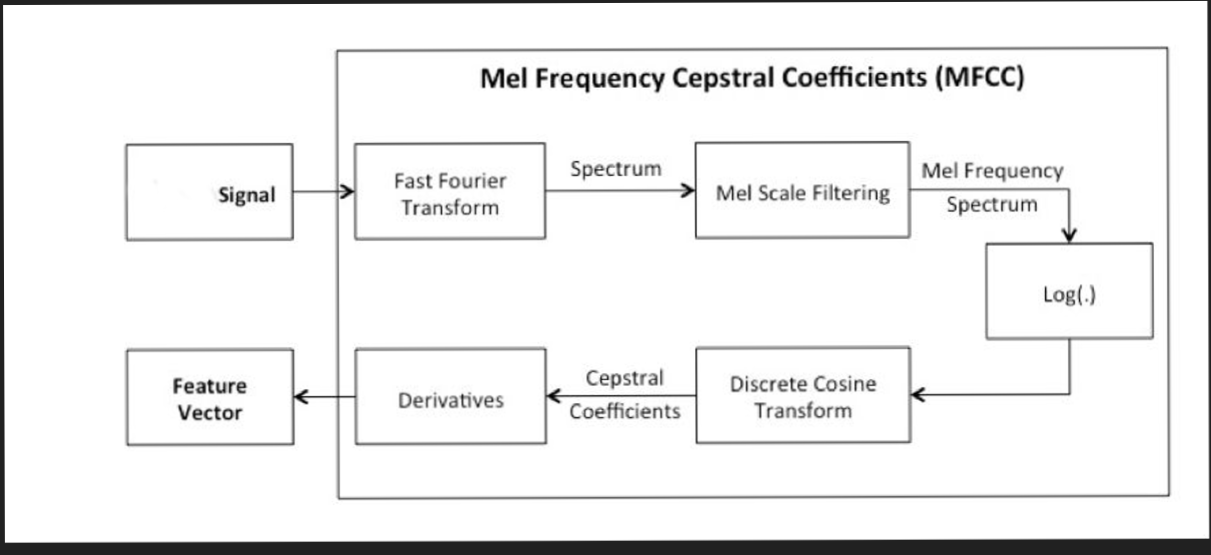
\includegraphics [scale=0.5]{mfcc.png}
\caption{mfcc algorithm}
\end{figure}
In the above figure as shown after the signal is sampled , first the fourier transformation is performed and the spectrum obtained is passed through the Mel Scale Filter. The output that we obtain is the Mel Frequency spectrum.
The log of the result is taken and a discrete Fourier transform is applied to the signal the result of this is the Mel Frequency Coefficient.
After performing the MFCC we have the signal saperated into different slots and each slots contain a the feature vectors. As suggested by johnson Lindestrauss we have taken 79 features per slot.The number of slots changes acoording to the length of the song.
\subsection{PCA} \textcolor{red}{Sahana}

\subsection{Content based similarity}
Beth and Ariel(\ref{logan}) presents a novel approach to compare songs based on their corresponding audio content. For each song in the dataset, they create a song signature. The song signature is generated based on k-means clustering of spectral features. The algorithm is summarized in figure (\ref{content}) below.

\begin{figure}[h]\label{content}
\center
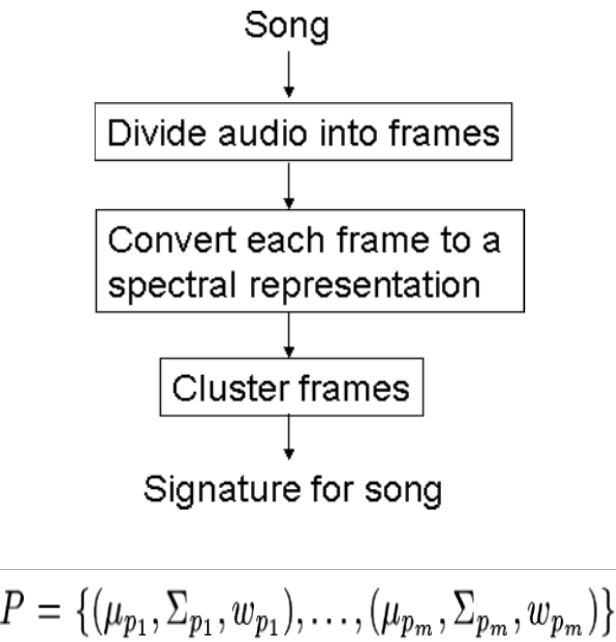
\includegraphics{fig1.png}
\caption{Content based similarity method}
\end{figure}

The first setup is to divide the audio into frames. Then, each frame is converted into its corresponding spectral representation. In order to generate the spectral representation we make use of mfcc algorithm which is explained in the previous sub section. The number of cepstrum coefficients was calculated based on the Johnson-Lindenstrauss lemma.

\subsubsection{Johnson-Lindenstrauss}
The idea behind Johnson-Lindenstrauss lemma
is that points in high-dimensional space can be projected onto low dimensional space while preserving the distance between the points. For a given dataset, the minimum number of dimension required to preserve the distance between the points is given by the formula $$ n > 8 * ln(m) * \epsilon ^ 2 $$ where $\epsion$ is a number between 0 and 1. For this project we have $$ n > 77$$ and hence the number of cepstrum coefficients that we have considered is 79.

\subsubsection{k-Means}
Once each frame is clustered into its corresponding we spectral representation, we cluster the frames using unsupervised k-Means clustering algorithm where the value of k is  fixed to 10. k-Means is a popular clustering algorithm used in data mining. It is often confused with k-nearest neighbour algorithm which makes use of supervised labels during the training phase in order to cluster the points. Given a set of n observations in a d dimensional space, k-Means aims to cluster the n dimension into k sets $S = {S_1,S_2,...S_k}$ where $ k \leq n$. The idea is to find the sum of distance functions of each point in the cluster to the K center. The equation is given by (\ref{kmeans}):

\begin{figure}[h]\label{kmeans}
\center
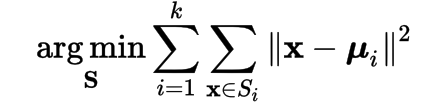
\includegraphics{fig2.png}
\caption{k-Means}
\end{figure}

\paragraph{}
After identifying the clusters, the mean, covariance and weight is calculated for each cluster. This set of values forms the signature of the song. This signature is used in order to compare two songs.

\subsection{Modified Gaussian Mixture} \textcolor{red}{Paria}

\section{Distance Metrics}
This section provides the different types of distance metrics that we used in our project. Distance metric is used to quantify the distance between two different songs in the song space. However, the distance metric is valid only on a low-dimensional sub space due to curse of dimensionality. For example: Consider a hypersphere. As the number of dimension increases the volume of hypersphere tends to zero. This phenomenon is also called as concentration of measure. In such a concentrated space euclidean or any type of distance is not meaningful. Hence, before calculating the distance we need to use dimension reduction as pre-processing step. The list of techniques that we experiment with for dimension reduction is discussed in the previous section (\ref{dr}).


\subsection{Minowski}
Minowski distance is considered as the generalization between euclidean distance and manhattan distance. This distance metric is used along with k-nearest neighbour for classification of points for songs which was reduced by content based similarity method. The reason why we used Minowski distance over other distance metric is based on experimentation. The distance between two n-dimensional point $ X = {x_1,x_2,...,x_n$ and $ Y = {y_1,y_2,...,y_n} $ is calculated as:
\begin{figure}[h]\label{kmeans}
\center
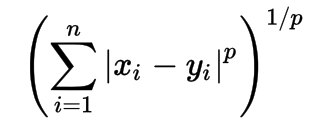
\includegraphics{fig3.png}
\caption{Minowski distance}
\end{figure}
\subsection{Earth Movers distance}\textcolor{red}{Abhijit}
\subsection{Euclidean distance}\textcolor{red}{Paria}
\subsection{Kullback-Leibler distance (KL) distance}\textcolor{red}{Paria}

	\section{Statiscal learning}
	In previous sections we discussed the projection of audio files into lower dimensional space. And we introduced the measure of distances we use to represent the distance between the new representations of the audio files. The next step is to build the classifier to these information for genre classification. We have implemented three classifiers that we explain here.
	\subsection{k-Nearest Neighbors}
	One of the common algorithms for classifying multi-class data is k-nearest neighbors (kNN). This algorithm simply finds the k closest data points to the testing point and determines which class owns the majority of points among these points. Therefore, the label for the testing data point would be the label of the majority of k closest data points.
	The following figure represents the kNN algorithm for $k = 3$. There are 2 classes in this example represented with blue and red color. The testing point is the black circle and because 2 out of 3 closest neighbors are in blue, the classifier will assign it to blue class.
	\begin{figure}[H]\label{kNN}
		\centering
		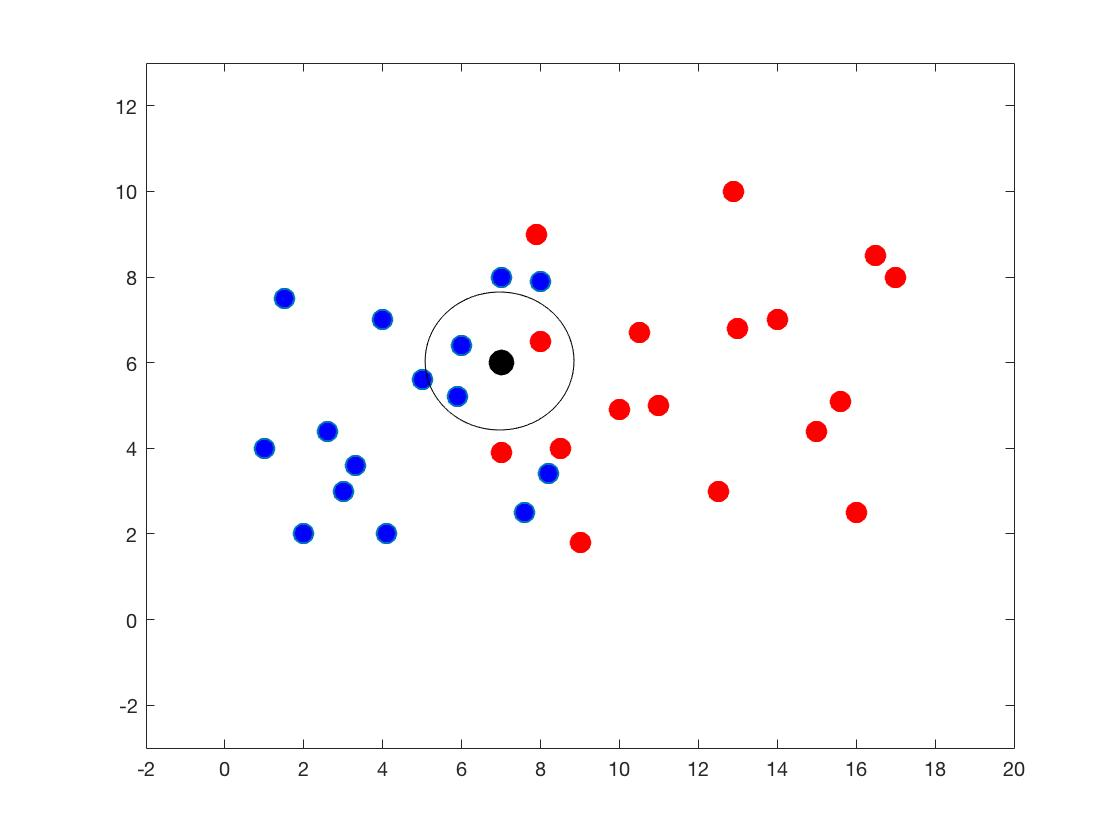
\includegraphics[width=.8\linewidth]{kNN.jpg}
		\caption{k-nearest neighbors}
	\end{figure}

\subsection{Modified-kNN}\textcolor{red}{Paria}

\subsection{Neural Network}\textcolor{red}{Sahana}
\section{Experiments}
%_________________________________________________________________
Describe the experiments, and include the confusion matrix. Discuss
the influence of the various parameters, and describe how the optimal
parameters were chosen. Include the computation time for your method. : \textcolor{red}{Sahana}
%_________________________________________________________________
\section{Discussion}
%_________________________________________________________________
Provide a critique of the approach and discuss any potential
improvement. Discuss the ability of your approach to classify
non-classical into the five remaining genres. \textcolor{red}{Abhijit}
\begin{thebibliography}{9}
	\bibitem{logan}\label{logan}
	Logan, B., & Salomon, A. (2001). A content-based music similarity function. Cambridge Research Labs-Tech Report.
\end{thebibliography}
\end{document}